\documentclass[12 pt,twoside]{article}
\usepackage{epsfig}
\usepackage{fullpage}
\usepackage[font={small,it}]{caption}

\begin {document}
\begin{center}

{\LARGE{\bf CCD Photometry and Star Flux Analysis}}

{\large Tim Kornish}

University of Montana

October 28th, 2014
\end{center}


\paragraph{Abstract}
Using three separate Landolt Standard stars with known magnitude of brightness (flux), the magnitude of three science stars can be calculated. Raw images can be manipulated with darks and flat images in order to reduce images to acquire only the signal counts from a star. Adjusting for quantum efficiency of the pixels in the CCD and subtracting bias and darks values there is a raw image. The Landolt standards are used to obtain a zero point because the commonly used Vega saturates the CCD to the point of being useless. With a zero point of magnitude acquired, the magnitude of each science star can be found. The magnitude is found from the equation: $m_1$ - $m_2$ = -2.5log$\frac{N_1/t_1}{N_2/t_2}$ which can be derived to give $m_1$  = -2.5log$\frac{N_1}{t_1}$ + ZP.  Where $\frac{N_1}{t_1}$ = Flux = $\frac{L_v}{4\pi d^2}$, $L_v$ is Luminosity, and d = distance.


\paragraph{Introduction}
Using the Johnson V filter, which transmits light in roughly 500 nm $<$ $\lambda$ $<$ 600 nm to allow only visible light to hit the CCD omitting IR and UV light. With a specific bandpass (frequency range) it is now possible to measure the Flux of a star. Flux, $F_v$ = $\frac{L_v}{4\pi d^2}$, $L_v$ is Luminosity, and d = distance, in $\frac{W}{m^2 Hz}$. Because the distance of all stars excluding the sun is so great, a handy unit converter is the Janksy where 1Jy = $10^{-26}$$\frac{W}{m^2 Hz}$. 

\ \

\indent
The number of counts in the CCD per exposure time t and area A can be shown as $N$ = ($A$)($t$) $\int_{v_1}^{v_2}$ $\frac{F_v\eta_v}{hv}$$dv$. With $F_v$ and $\eta_v$ varying lowing in the waveband the integral can be approximated as $F_v$ $\approx$ $ \frac{N hv}{A t \eta_v \Delta v}$. where $F_v$ $\alpha$ $\frac{N}{t}$. 

\ \

\indent
Now plugging the flux into the equation to find magnitude of the star: $m_v$  = -2.5$log_{10}$$\frac{F_v}{F_{v,0}}$ where $F_{v,0}$ is the reference flux that defines the magnitude. In this case and many others $F_{v,0}$  is of the star Vega with a set $m_v$ = 0.0 at all frequencies.





\paragraph{Observations}

\indent
Observations of several stars were performed on 9-16-2014 using a 0.4m diameter telescope. During civil twilight, several flat images were taken pointed at evenly illuminated sky. Beginning at Astronomical twilight images were taken of three science starts and three Landolt Standard stars. Nine images were taken of each star in a slightly different place on an Apogee Alta U47 1024 x 1024 pixel CCD. This was done to account for damaged or not properly functioning pixels. Each of these pixels having an area of 13 x 13 microns. The CCD was cooled to $-20 \pm 0.1\,^{\circ}{\rm C}$ going a dark current of only 0.2 electrons/pixel/second.

\ \

\indent
One Landolt star had images taken with a very low airmass and then another with a much higher airmass later into the night as the star dropped closer and closer to the horizon. The other two Landolt standard stars were only viewed at one point during the night. The three Landolt stars observed were: GSC 0511:2062; GSC 0447:0541; and GSC 0478:1575, which was observed both at the beginning of the observation run and at the end. These stars are used to calibrate the brightness (flux) of the science stars using known magnitude of these stars. All Landolt stars were imaged with and exposure of 20 seconds due to their magnitude. 

\ \

\indent
The science stars are imaged and use the Landolt standards to find a zero point and acquire a magnitude of flux of these three stars. The three science stars chosen were: GSC 1051:1778; GSC 0108:4548; and GSC3184:1316. GSC 1051:1778 and GSC3184:1316 both had low exposure times due to their magnitude. GSC 1051:1778 was exposed on the CCD for one second and GSC3184:1316 was exposed for three seconds. GSC 0108:4548 has a much lower flux and needed a 20 second exposure to saturate the CCD to equivalent counts as the other two science stars.

\ \

\indent
At the end of observing starts, several darks were taken at exposure times equal to exposure times for each star. Eleven Dark were taken for one, three, and twenty second exposures. These darks will later be used to manipulate the raw image of each star recorded.



Using methods in previous experiments to account for quantum efficiency, read noise, and gain of CCD. Gain and read noise of CCD being 1.39 electrons per DN and 8.42 electrons respectively.

\paragraph{Analysis}

\begin{center}
\begin{figure}[!hb]
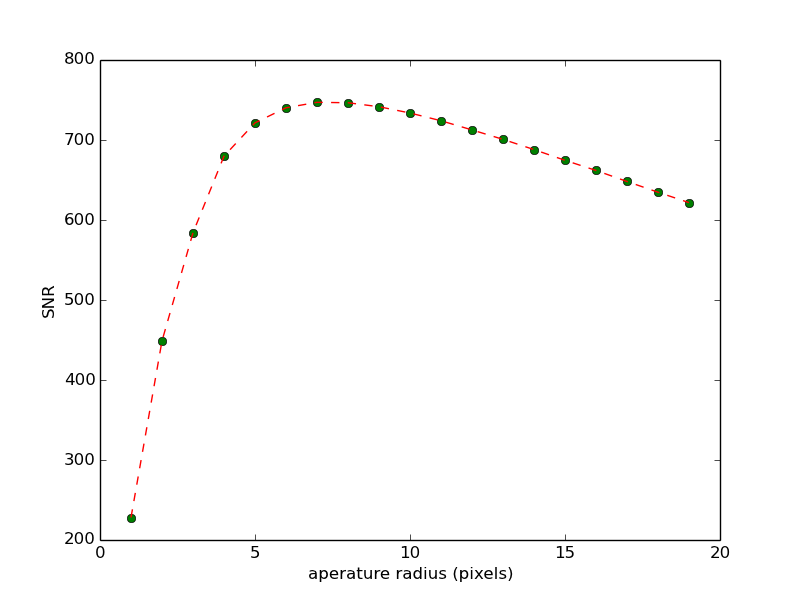
\includegraphics[scale=0.5]{figure_1.png}
\caption{\small SNR vs Aperture size: The plot shows what radius that will maximize the signal-to-noise ratio for our measured starlight. The maximum is approximately eight pixels in radius. Even if this radius won't capture all the light from the star, it is still the ideal radius. This radius will only work for the star we chose to observe. To find a radius that will fit all stars, the median best aperture radius is chosen over the mean.}
\end{figure}
\end{center}

The signal-to-nose ratio is given by the equation: 
\begin{center}
$SNR$ = $ \frac{g * N_{star}}{(g  *  N_{star} + n * g * N_{sky} + n * RN^2)^{1/2}}$
\end{center}

\noindent where g is gain, $N_{star}$ is the total star light counts in the aperture. RN is the read noise, n is all the pixels inside of the aperture, and $N_{sky}$ is the number of background counts in any pixel due to light reflected off the atmosphere, other stars, or the moon. $N_{star}$ and n are dependent on the aperture radius which is chosen from figure 2.

\begin{center}
\begin{figure}[!hb]
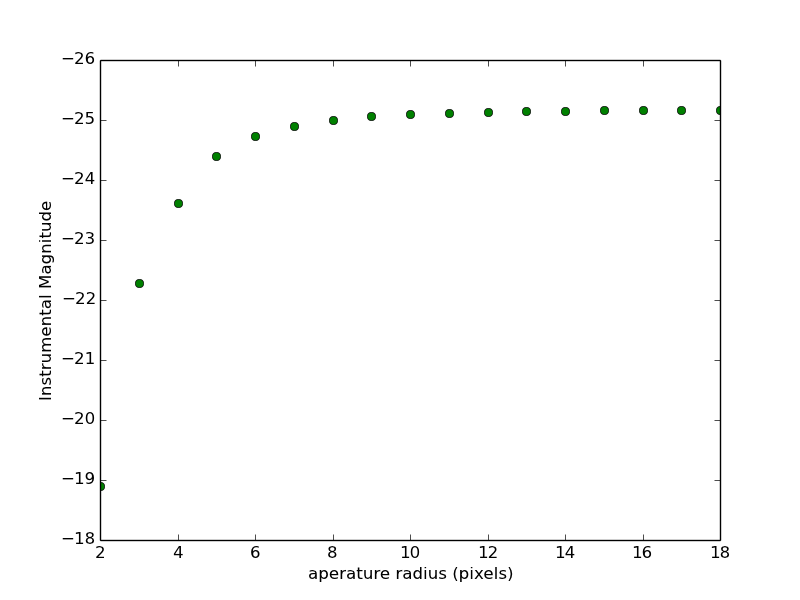
\includegraphics[scale=0.5]{figure_2.png}
\caption{\small Curve of Growth: This shows the intrinsic magnitude growing more negative as more and more DN from the star are counted inside an increasing radius. The magnitude grows rapidly while the aperture is still inside the body of the star but plateaus once leaving the edge of the star. The curve appears to continue growing at a very minimal rate due to noise being counted. This plot shows that after a certain radius most of the stars light has been counted. This occurs at nine-ten pixels in radius. }
\end{figure}
\end{center}

The median of the best radii for all images is found to be nine pixels, but because of the FWHM in some images was so large, a better radius of 12 pixels is chosen for calculating the instrumental magnitudes. By changing the radius to 12 there is a loss in precision because extra DN are being counted from the background, but in exchange there is an increase in accuracy. The SNR decreases very slowly after there maximum so only a low amount of precision is lost for a larger gain in accuracy from increasing the aperture size. 

\begin{center}
\begin{figure}[!hb]
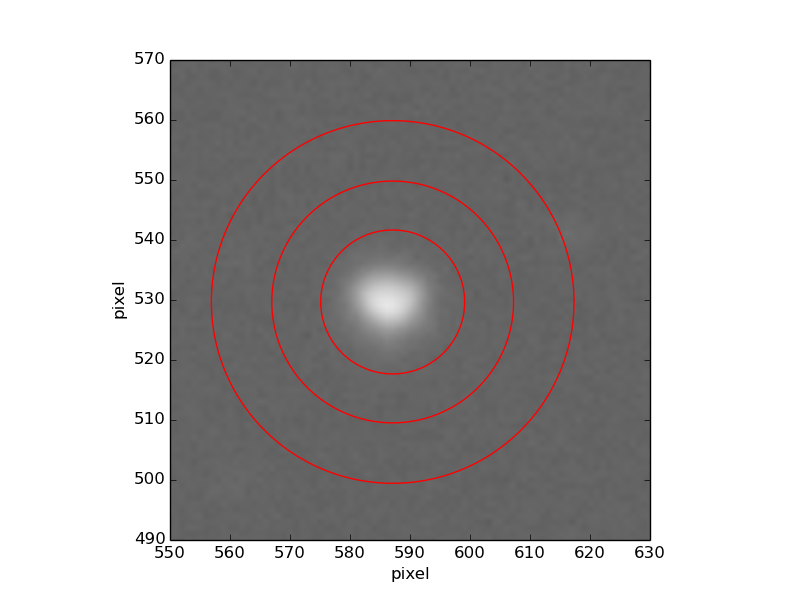
\includegraphics[scale=0.5]{figure_4.png}
\caption{\small Star with an aperture and annulus surrounding it. The aperture and annulus are centered around the star for higher precision of counting the the amount of light from the star. The aperture (center circle) is specifically for summing the amount of light from the star. The annulus (two outer circles) are used to calculate a median sky count. The ideal radius of the aperture is maximizing the SNR, but in this case it is more useful to use a larger radius.}
\end{figure}
\end{center}

To calculate the magnitude of the stars observed, the magnitudes of another star must first be known. Using Landolt Standards with carefully measured magnitudes by other astronomers, a zero point (ZP) can be calculated. The original equation of: 
\begin{center}
$m_1$ - $m_2$ = -2.5log$\frac{N_1/t_1}{N_2/t_2}$  (1)

can be derived into
 
$m_1$  = -2.5log$\frac{N_1}{t_1}$ + ZP.              (2)
\end{center}
The measured ZP of the landolt stars becomes 20.774066 $\pm$ 0.028066. With a known ZP, equation 2 can now be used to find the magnitude of the stars being observed.
 


\pagebreak
\paragraph{Results}

Through several manipulations the of the raw images to find the magnitude of the three science stars. 

star 1: GSC10511778  has a magnitude of 5.305881 $\pm$ 0.028066

star 2: GSC1084548    has a magnitude of 9.892144 $\pm$ 0.028066

star 3: GSC31841316: has a magnitude of 7.849142 $\pm$ 0.028066

\ \

\noindent Actual values of these stars measured from other astronomers off Simbad database show:

star 1: GSC10511778  has a magnitude of 5.89

star 2: GSC1084548    has a magnitude of 10.38 

star 3: GSC31841316: has a magnitude of 8.55 

\ \ 

These results are not accurate or precise holding in the true magnitude value in their uncertainties. This can be do to a large number of issue. First is the issue of the atmosphere which causes turbulence creating a larger full width-half max (FWHM). A second issue is the light pollution due to observing in the center of a small city that radiate light and can be reflected into the telescope off the atmosphere. The moon can also play an affect on observation along with the airmass that the star is being observed through where 1 airmass is most preferable. Weather can play a major role including wind, humidity, etc. All the measurements gave precise magnitudes but were all offset from the actual value by approximately 0.5-0.6.

\paragraph{Conclusion}

With different stars different aperture sizes are preferable to get the most accurate and precise image analysis as possible. Maximizing the SNR may often seem to give the best aperture radius but as stated sometimes a trade in precision for higher accuracy. As shown in the results the magnitudes were not accurate but may have been even less accurate if a smaller aperture radius is chosen. 

\ \

A very important part of this experiment was to show the importance of choosing the proper aperture and annulus size. A large enough aperture to capture all the star light but not continuing far beyond collecting background.

\ \

The Annulus is very import in order to help delete the counts reflected of the atmosphere off the raw image. Without the annulus or aperture, the results of magnitude would become very skewed.














\end {document}